
\section{Implementering}
\subsection{Model}
Modellen er nu lavet så det er muligt at vælge mere end én spiller. I både \textit{GameSingleplayer} og \textit{GameMultiplayer} findes en timer hvor det dog kun er i Singleplayer-spillet at timerens opdateringsinterval formindskes efter hvert femte samlet æble. Slangen er stadig defineret som en ArrayList i klassen \textit{Snake}, hvor også dens [.......................]

\subsubsection{Multiplayer}

\subsection{View (Brugergrænseflade)}
Ændret siden simpel: Tilføjede scener. Brug af importerede billeder. Optegning af slange efter bevægelse.


Når \textit{View}-klassen konstrueres, opretter den i sin constructor \textit{ViewAudio}-, \textit{ViewMenu}-, \textit{ViewHeader}- og \textit{ViewControls}-objekter. \textit{ViewAudio}-klassen står for spillets lyde, der spilles efter slangens handlinger i spilscenen hvis klassens Boolean felt \textit{muted} er falsk. \textit{ViewHeader} er en topbar, som indeholder spillets titel, tastatur-genveje og en JButton, der viser om lyden er slået til eller fra og som ligeledes kan bruges til at slå lyden til eller fra. \textit{ViewMenu}-panelet indeholder JButtons som giver spilleren adang til spillets scener: Singleplayer, Multiplayer og Controls - der fører til hjælpescenen \textit{ViewControls}. Desuden har den også en \textit{Quit}-knap, som fungerer som vinduets kryds i hjørnet. Når \textit{View} oprettes i \textit{Driver}-klassen og sættes til visible, kører den først \textit{showMenu}-metoden, der tilføjer \textit{ViewHeader}-panelet og \textit{ViewMenu}-panelet. Disse skiftes kun ud med andre paneler gennem input fra spilleren, når spilleren bevæger sig rundt i spillet. Dette sker med \textit{View}s \textit{setFrameComponents} metode, der tager to komponenter som parametre, hvorefter Frame'n skifter dens nuværende indhold ud med de to nye paneler. Frame'n bruger \textit{BorderLayout}, der gør det simpelt at placere et header-panel øverst, og det ønskede scene-panel nedenunder. Alle andre view-klasser er efterladt med standard-layoutet \textit{FlowLayout}, da deres komponenter skal placeres i specifikke koordinater. Dette gøres med \textit{setLocation} der definerer komponentets præcise placering ved x- og y-koordinater. Når spilleren ændrer vinduets størrelse, er deres koordinater dog ikke altid bevaret hvis komponenterne f.eks. altid skal ligge i midten af vinduet. Disse kald på \textit{setLocation}-metoden er derfor placeret i panelernes \textit{paintComponent}-metode da, denne køres hver gang vinduet skaleres. Koordinaterne beregnes derved påny hver gang vinduet skaleres, og komponenterne kan derfor altid få de rigtige koordinater. Denne metode er brugt til alle billeder, JComponents og tekst der oprettes eller tegnes.

((((((((((Klikkes der på \textit{Singleplayer}- eller \textit{Multiplayer}-knappen, skiftes menu-panelet ud med henholdsvis \textit{ViewOptioinsSinglePlayer} eller \textit{ViewOptionsMultiplayer}, der hver viser indstillings-scenerne for hver game-mode. Klasserne har superklassen \textit{ViewOptions}, der tegner baggrunden, skriver tekst, opretter input-felter til valg af bane, konsturerer sværhedsgradsknapper og play- og back-knapper. Underklasserne opretter selv deres farve-knapper, da der for multiplayer skal være otte knapper i alt, mens singleplayer kun har fire forskellige knapper. Gå man videre herfra vha. play-knappen, skiftes panelerne endnu engang ud med enten \textit{ViewHeaderSingleplayer} og \textit{ViewBoardSinglePlayer} eller \textit{ViewHeaderMultiplayer} og \textit{ViewBoardSingleplayer} der er underklasser til \textit{ViewHeader} og \textit{ViewBoard}.)))))) - Design?


(((((((I klassen \textit{ViewBoard} tegnes grafikken til spillet. Her er lagt specielt vægt på, at felternes størrelse passer til spillerens ønskede bane-størrelse og spillerens ønskede vinduesstørrelse samtidig med at bevare deres kvadrate form. Metoden \textit{getFieldSideLength} beregner ud fra disse to størrelser den størst mulige længde og højde af et enkelt felt og returnerer derefter den mindste af de to værdier. På denne måde kan feltet være kvadratisk og passer med sikkerhed på begge led af vinduet. Denne \textit{getFieldSideLength}-metode kan nu bruges til at bestemme størrelsen af og tegne banen, slangen og æblet, så de passer til vinduets størrelse. Da disse tegnemetoder bliver kaldt fra \textit{paintComponent}-metoden, der køres igennem konstant under spillet og når vinduesstørelsen ændres, har spillets komponenter altid en passende størrelse.))))))))))- gentaget?
Når spilleren færdiggør spillet enten ved at tabe eller vinde, tegnes \textit{Game Over}-skærmen ved en gennemsigtig rektangel, med \textit{Final Score} og JButtons, der giver mulighed for at gå tilbage til menuen eller spille igen.
Udover bane-størrelse er det også muligt at vælge slangens farve. Når en farve er valgt tjekkes der i \textit{drawSnake}-metoden i \textit{ViewBoard}-klassen om farven har været valgt før. Hvis ikke tilføjes den nye farve til ArrayListen \textit{snakeColors}, mens alle billederne som udgør slangen farves og bruges til at tegne slangen. Hvis farven har været valgt før, behøves billederne ikke at farves igen, men kan hentes i hvert billedes egen ArrayListe. Billederne farves ved at køre hver enkel pixel igennem ved en indlejret for-løkke og derefter give det en anden farve defineret ved tre heltal givet som parametre til \textit{colorSnakeImage}-metoden, der farver den givne pixel, hvis dens farve ikke er svarende til slangens øjenfarve.

\subsection{Control (Styring)}
Ændret siden simpel: Mute, pause, escape, enter.

For at give spilleren valgfrihed er der til mange funktioner både implementeret en JButton og en tilhørende genvej gennem tastaturet. Fra tastaturet er der blevet implementeret følgende genveje: Mute-knap (M), pause-knap (P), menu-knap (Esc), tilbage-knap (Backspace) og (re)start-knap (enter/space). \textit{Control}-klasserne [extends] \textit{KeyAdapter}, der registerer tastatur-input, og implementerer \textit{ActionListener}, der registrerer tryk på JButtons. Disse klasser tilføjer \textit{KeyListeners} til \textit{View}-klassen, og \textit{ActionListener} til hver enkel knap, der har funktioner i ActionListenerens tilhørende klasse. Individuel kontrol over de forskellige knapper fås ved at sætte en unik \textit{ActionCommand} til hver enkel knap, der derefter kan tjekkes for i ActionListeneren abstrakte metode \textit{actionPerformed}. Det er her også nødvendigt efter knappetryk at bruge \textit{requestFocus}-metoden på \textit{View}-klassen, da spillet efter knappetryk, får et nyt fokus, hvilket betyder, at tastatur-inputtet ikke opfattes af spillet.
Især når \textit{View} oprettes, bruges \textit{setFocusable}- og \textit{requestFocus}-metoderne, eftersom tastatur-input allerede skal være brugbart når spillet åbnes på grund af \textit{mute}-funktionen.

\textit{Control}-klassen er en global klasse, der står for kontrollen overalt i spillet. Dvs. muligheden for at slå lyden til eller fra eller vende tilbage til menuen. Når enten (M) eller lydknappen trykkes på, sættes \textit{ViewAudio}-klassens boolean 'mute' til det modsatte af det den i forvejen var, mens \textit{ViewHeader} (eller dens underklasser) notificeres for at opdatere lyd-ikonet. [INSERT PIC]
\textit{ControlBoardMultiplayer} og \textit{ControlBoardSingleplayer} indeholder metoden \textit{actionPerformed}, der genstarter eller går ud af spillet når spilleren trykker på 'Play Again'-knappen eller 'Menu'-knappen. Klasserne indeholder også KeyEvents, som kalder på en \textit{move}-metode i \textit{GameSingleplayer} eller \textit{GameMultiplayer}, der får slangen til at bevæge sig, når spilleren trykker på tastatur-tasterne, som styrer slangen. Klasserne indeholder også KeyEvents'ene (P), der fryser spillet og (ENTER)/(SPACE), der fungerer som 'Play Again' knappen.

\textit{ControlOptions}, der er en abstrakt klasse implementeret af \textit{ControlOptionsSingleplayer} og \textit{ControlOptionsMultiplayer}, styrer knapperne i indstillings-scenerne. Før spillets start kan spilleren som tidligere nævnt - udover at vælge farve og sværhedsgrad - vælge banestørrelsen. Denne funktion er indbygget vha. to \textit{JFormattedTextFields} der har fået en \textit{Formatter}, som begrænser inputtet til højst et tre-cifret tal. Dette begrænser spillerens mulighed for at indtaste en ugyldig størrelse. Trykkes på en af farve-knapperne eller sværhedsgrads-knapperne, optegnes den vha. JButton-metoden \textit{setBorder} med en tyk kant, for at vise at den er aktiv, mens kanterne på de andre knapper fjernes med \textit{setBorderPainted(false)}. Trykkes på en farveknap, sendes farven til \textit{ViewBoard}s \textit{setSnakeColor}-metode, der derefter bruger farven som beskrevet tidligere. Trykkes på en sværhedsgradsknap, sættes  en 'Difficulty' enum til den valgte sværhedsgrad. Denne bruges når 'Play'-knappen trykkes eller der trykkes (ENTER). 'Play'-knappen kalder på den implementerede abstrakte metode \textit{playAgain}, som først tjekker om tekst-felterne for bane-størrelsen er tomme, da der så printes en fejlmelding. For ikke at gøre det for svært for spilleren at indtaste en gyldig værdi, ses der bort fra eventuelle mellemrum før, i eller efter tallene. Dette gøres med metoden \textit{getInput} i superklassen, der fjerner alle mellemrum. Der undersøges derefter om tallene ligger mellem 5 og 100. Hvis dette er tilfældet, sættes bane-størrelsen vha. game-klassernes \textit{setBoardSize}-metodem, sværhedsgraden sættes med \textit{setSpeed}-metoden, spillet nulstilles (i tilfælde af at det har været startet før) og startes.

(((((((Da tekstfelterenes \textit{Formatter} får deres caret til at sætte sig i starten af tekstfeltet selvom spilleren trykker et andet sted i feltet, implementerer \textit{ViewOptions}-klassen en \textit{FocusListener}, der har de abstrakte metoder \textit{focusGained} og \textit{focusLost(...)}. I \textit{focusGained} oprettes )))))).

\section{Udviklingsproces}
\subsection{Control}
Diskussion: Opdeling af controlklasser

\subsection{Model}
\subsubsection{Menu}
Forklaring af

\subsubsection{Multiplayer}
Singleplayer og multiplayer

\subsubsection{Automatisk bevægelse}
Timer og acceleration


\subsection{View}
\subsubsection{Tegning af slangen}
Ændret siden simpel: Undersøgelse af slangens led

I Simpel Snake kan spilleren ud fra slangens krop se hvor han har været, men ikke hvilken vej han har bevæget sig, idet de udfyldte felter er fyldt helt ud til kanten[FIG HENVISNING]. Slangens udseende kan derfor forbedres ved at vise slangens bevægelsesretning og retningsskift i hver enkel del af dens krop og generelt erstatte alle firkanterne, med mere beskrivende billeder [FIG HENVISNING]. Dette giver seks mulige udseender for hver enkel del af slangen udover hovedet og enden af halen, der hver findes i fire versioner afhængig af retningen, som spilleren vælger for hovedet, eller retningen af kropsdelen lige før halen. Kropsstykkerne imellem er dog ikke kun afhængig af retningen af stykket lige før eller lige efter, men begge dele. Den vandrette del og den lodrette del af slangen bestemmes let ved at undersøge om stykket, der skal tegnes ligger i samme række eller kolonne som stykkerne før og efter. Slangens hjørnestykker bestemmes på en mere indviklet måde, da stykket og dens tilgrænsende stykker aldrig ligger i samme række eller kolonne, men derimod kan ligge i fire forskellige forhold til hinanden (Se figur 3.1). I figur \ref{fig:corner1} ligger de tilgrænsende felter lige under og til højre for hjørnet, men dette gælder f.eks. ikke for figur \ref{fig:corner3} hvor det ene stykke ligger lige under, mens det andet stykke ligger til venstre for hjørnet uden at grænse op til dens venstre side, der ellers ville give hjørnestykket spejlvendt i y-aksen. Da felterne ligger i en XXXXX-liste sorteret efter slangens opnåede dele, sammenlignes et felt med feltet før og efter det i listen. Da stykket foran og bagved uden påvirkning på hjørnestykket kan bytte plads, findes der altså otte situationer for et enkelt hjørnestykke. I alt tjekkes der derfor - for kroppen alene - 34 mulige forhold mellem et stykke og dens to tilgrænsende stykker.
\linebreak

I \textit{ViewBoard}-klassen er der lavet en \textit{drawSnake}-metode, der består af en del if-statements, for hvilket figur af slangen, der skal bruges i en bestemt retning. I \textit{snakeCorner}-metoden returnerer den en lang boolean \textit{isCorner}, som tidligere har været kopieret 4 gange for de fire retninger, men som nu er blevet simplificeret med en masse variable til den samme boolean. Måden det blev gjort på, var at finde et mønster i de fire lange booleans før og så indsætte 12 forskellige varibale, der gjorde det muligt kun at kalde en boolean. På samme tid kører programmet ikke alle if-else-statements igennem hver gang den skal lave et hjørne, men kun det hjørne som bliver kaldt. Variablerne kan enten have værdien 0, 1, -1, lastColumn eller lastRow. Da det specifikke hjørne skal dukke op et bestemt sted alt efter hvor på banen slangen befinder sig.
De første to rækker kode af \textit{isCorner}, fortæller om når slangen er placeret midt på banen (se figur \ref{fig:corner1}), og drejer til den specifikke retning, så må det foranliggende (front) og bagvedliggende stykke (behind) ligge et bestemt sted, som enten getColumn()+1 eller getColumn()-1 og på samme måde getRow()+1 eller getRow()-1. I de to næste ligner kode i \textit{isCorner} beskriver den, hvis slangen er placeret på den sidst række (altså i bunden af banen) og går gennem torussen, så den ender øverst i banen (se figur \ref{fig:corner2}).
De to næste linjer kode er på samme måde, når slangen ligger yderst til højre eller venstre og går gennem torussen (se figur \ref{fig:corner3}).
De to sidste linjer kode er til, når slangen går gennem torussen to steder i et af hjørnerne. Altså hvis slangen f.eks. er nede i højre hjørne, går gennem torussen ved at gå ned ad, og straks til højre gennem torussen igen (se figur \ref{fig:corner4}). 
Derved er alle hjørne-situationer gennemgået.
Man kan se et mere detaljeret billede af snake-kroppen i Appendix (Bilag A).
\begin{figure}[h]
	\centering
	\graphicspath{ {pics/} }
	\caption{}
	\subfloat[Corner 1]{\label{fig:corner1}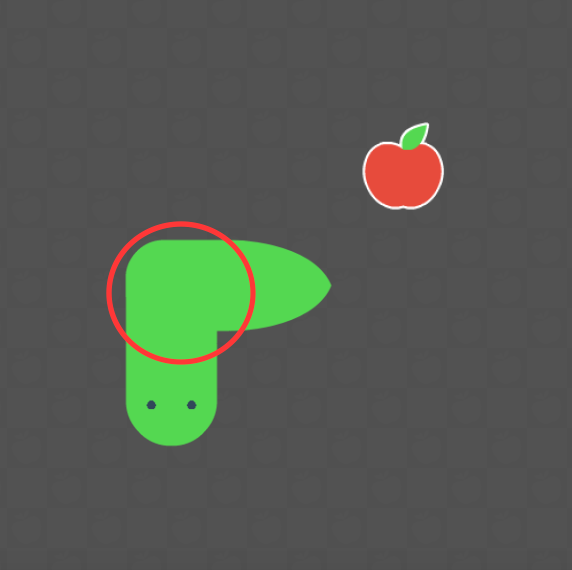
\includegraphics[width=0.15\textwidth]{Corner1.png}}
	\hspace{0.05\textwidth}
	\subfloat[Corner 2]{\label{fig:corner2}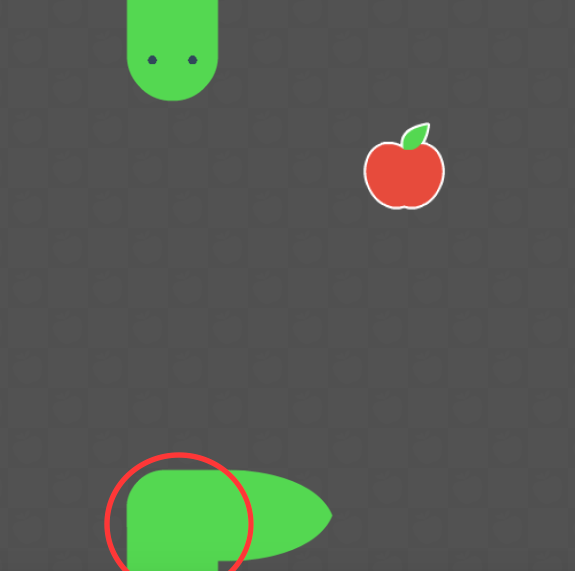
\includegraphics[width=0.15\textwidth]{Corner2.png}}
	\hspace{0.05\textwidth}
	\subfloat[Corner 3]{\label{fig:corner3}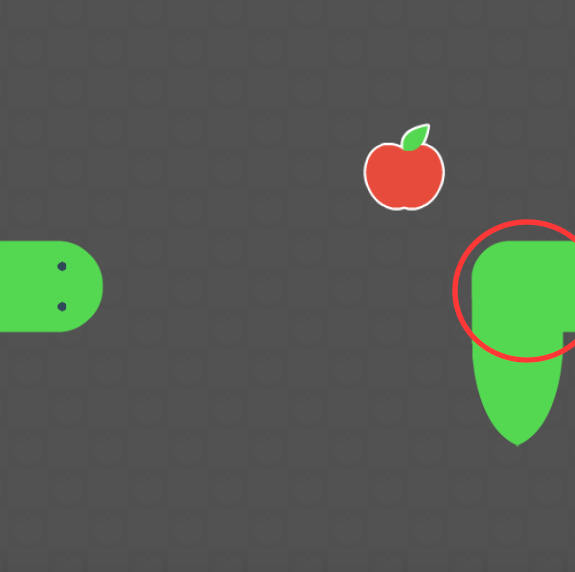
\includegraphics[width=0.15\textwidth]{Corner3.png}}
	\hspace{0.05\textwidth}
	\subfloat[Corner 4]{\label{fig:corner4}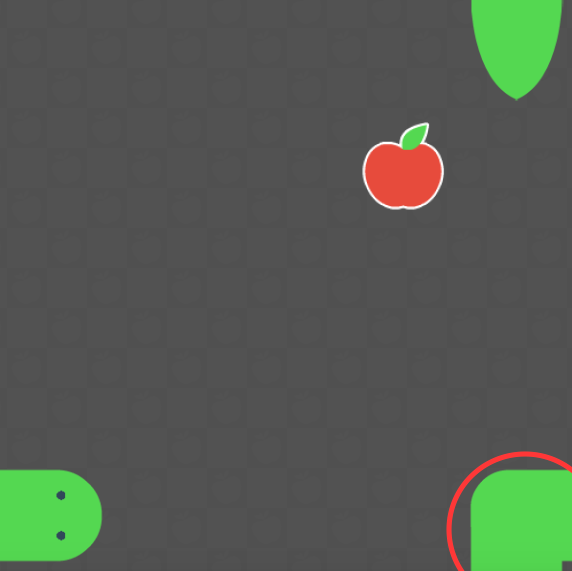
\includegraphics[width=0.15\textwidth]{Corner4.png}}
\end{figure}

\subsubsection{Lyd}

Som en mindre tilføjelse til spillet er lyd tilføjet i form af Audio-klassen. Funktionerne i Audio-klassen bruges til individuelt at spille 	
